% !TeX root = ../Book3.tex
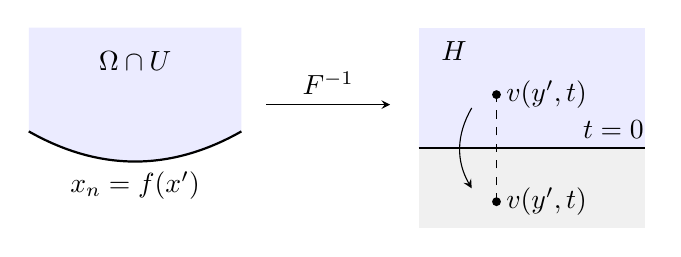
\begin{tikzpicture}[x=.9cm,y=.85cm,>=stealth]
	\fill[blue!8] (0,.25) .. controls (1,-.35) and (2,-.35) .. (3,.25) -- (3,1.8)--(0,1.8)--cycle;
	\draw[thick] (0,.25) .. controls (1,-.35) and (2,-.35) .. (3,.25);
	\node at (1.5,1.3) {\(\Omega\cap U\)};
	\node[below] at (1.5,-.2) {\(x_n=f(x')\)};
	\draw[->] (3.35,.65)--(5.1,.65) node[midway,above] {\(F^{-1}\)};
	\fill[blue!8] (5.5,0) rectangle (8.7,1.8);
	\fill[gray!12] (5.5,-1.2) rectangle (8.7,0);
	\draw[thick] (5.5,0)--(8.7,0);
	\node[above] at (8.25,0) {\(t=0\)};
	\node at (6,1.45) {\(H\)};
	\draw[dashed] (6.6,-.8)--(6.6,.8);
	\fill (6.6,.8) circle (1.6pt) node[right] {\(v(y',t)\)};
	\fill (6.6,-.8) circle (1.6pt) node[right] {\(v(y',t)\)};
	\draw[->] (6.25,.6) to[bend right=30] (6.25,-.6);
\end{tikzpicture}
